\chapter{Collaboratively running experiments}
\begin{quote}
\emph{People have creative scientific questions and folk theories;
yet most lack the expertise to investigate them. How might
people transform their questions into experiments that
inform both science and their lives? This chapter introduces
the Galileo system}; it provides procedural support using
three techniques: 1) experimental design workflow that
provides just-in-time training; 2) review workflow with
scaffolded questions; and 3) automated routines for data
collection. We present three empirical investigations: a
between-subjects experiment with students, a study with
online volunteers across 16 countries, and a deployment
with online volunteers across 8 countries. Procedural
support yielded higher-quality experiments than watching
lecture videos. People generated structurally-sound experiments
on personally meaningful topics and ran them with
participants from around the world.
\end{quote}

\begin{figure}[h] 
  \centering
  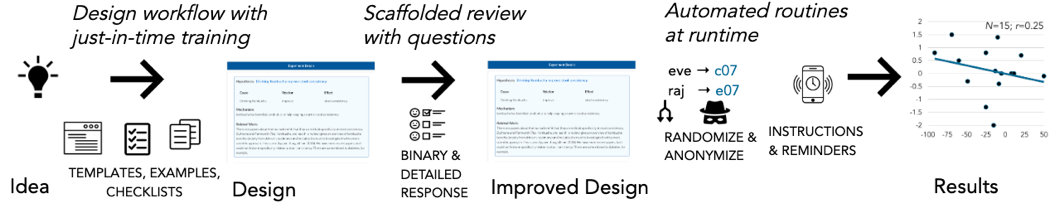
\includegraphics[width=0.9\textwidth]{figures/galileo/galileo-1}
  \caption[Galileo enables anyone to design and run experiments to test their intuitions]
{Galileo enables anyone to design and run experiments to test their intuitions. Experiment creators can invite anyone to review and participate in the experiment. Participants from around the world join experiments, follow instructions, and provide data in response to automated data collection reminders.\index{galileo-1}}
  \label{fig:galileo-1}
\end{figure}

\vspace{0.25in}

%%%%%%%%%%%%%%%%%%%%%%%%%%%%%%%%%%%%%%%%%%%%%%%%%%%%%%%%%
\section{Experience to Experiments: Self-tracking Offers Insights but Not Causality}
People have questions about their health, but lack the expertise and resources to scientifically
investigate them. These concerns are especially acute when multiple factors interact. Despite
knowledge gained from lived experiences, people lack the procedural tools to gain the causal
knowledge they seek. Many self-tracking efforts suffer from structural flaws that prohibit people
from actually learning what they'd like to know~\cite{Choe2014, Li2010a}. A frequent error is mistaking correlation
for causation~\cite{Munroe2009}. People falsely believe that when one event follows another, the initial event is
the cause: post-hoc ergo propter hoc. At the same time, professional science suffers from structural
biases. By creating controlled experiments (as opposed to tracking oneself), people can test their
intuitions at a larger scale, potentially unearthing novel results. How can we train people in designing
and running experiments to answer their personally-meaningful questions?

Scientific experimentation features technical requirements and contextual choices that are inscrutable for a lay individual yet necessary for success~\cite{Martin2007}. While professional scientists and commercial ventures run experiments every day, with notable exceptions~\cite{Cooper2010, Lewis2016}, empirical papers from non-professionals are vanishingly rare. This biases the questions asked, studies run, and knowledge created~\cite{crawford2017politics,Henrich2010a}. People have questions about their health, but lack the expertise and resources to scientifically investigate them. Broadening the pool of experimenters could help people investigate their curiosities, develop solutions to improve health and performance, and assist institutional researchers.

The main contribution of this chapter is \textit {demonstrating that online volunteers can collaboratively perform scientific experimentation}. It does so in two main ways: 1) procedural support for acquiring domain expertise using three techniques: experimental design workflow that provides just-in-time training, review with scaffolded questions, and automated routines for data collection; and 2) the Galileo social computing system that instantiates procedural support for citizen experimentation (Figure~\ref{fig:galileo-1}). 

Three empirical investigations tested Galileo's approach. First, a controlled between-subjects experiment with 72 participants found that procedural support yielded significantly higher-quality experiment designs than lecture videos. Second, a deployment across 16 countries found that people generated structurally-sound experiments on personally meaningful topics. Third, in a field deployment, online users from three communities---kombucha, Open Humans, and beer---across 8 countries demonstrated that people designed, iterated on, and ran week-long experiments.

%%%%%%%%%%%%%%%%%%%%%%%%%%%%%%%%%%%%%%%%%%%%%%%%%%%%%%%%%
\section{The Galileo Experimentation platform}

Galileo introduces a system for end users to design experiments, get them reviewed, and run them with interested participants. It provides procedural support for these steps, an online collaboration platform, and automated data collection and reminders.

Despite a predetermined goal and a formalized process, experimentation requires making contextually-appropriate decisions~\cite{Martin2007}. Good experiment design is inherently user centered; designers need awareness of others' interpretation of their ideas and asks. Providing feedback on experiment designs requires knowing the success criteria and how to help improve.

%\begin{wrapfigure}[23]{r}{0.5\textwidth}
%%\vspace{-0.25pt}
%  \centering
%  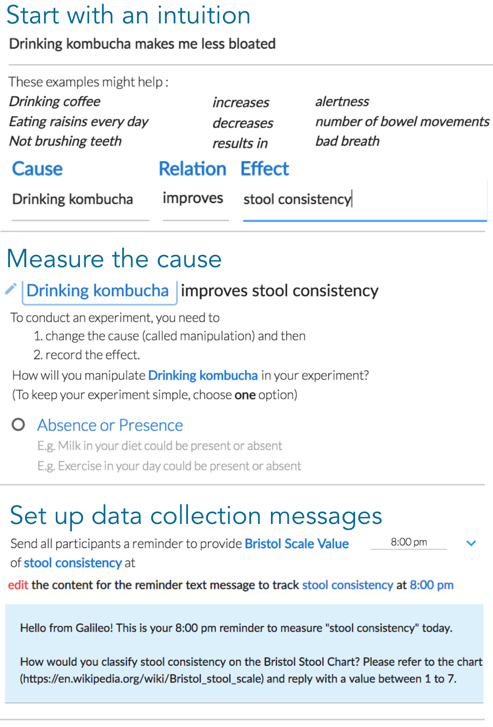
\includegraphics[width=0.48\textwidth]{figures/galileo/galileo-2-design}
%  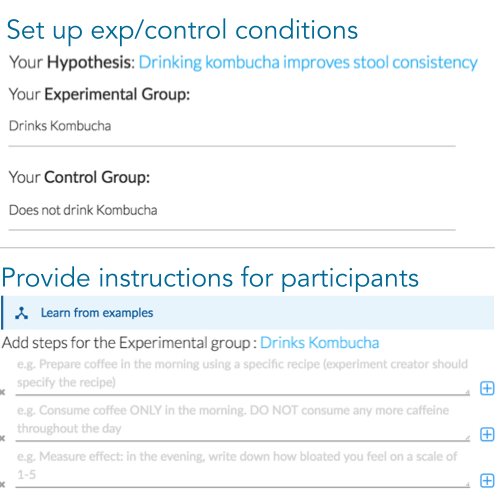
\includegraphics[width=0.48\textwidth]{figures/galileo/galileo-2-design-2}
%  \caption[Galileo's design module helps people transform intuitions into experiment designs]
%{Galileo's  design module helps people transform intuitions into experiment designs. It walks people through 1) converting an intuition to a hypothesis, 2,3) providing ways to manipulate/measure cause and effect, 4-5) specifying control and experimental conditions, and (not shown) providing inclusion/exclusion criteria.\index{galileo-2}}
%  \label{fig:galileo-2}
%\end{wrapfigure}

\begin{figure}[h]
%\vspace{-0.25pt}
  \centering
  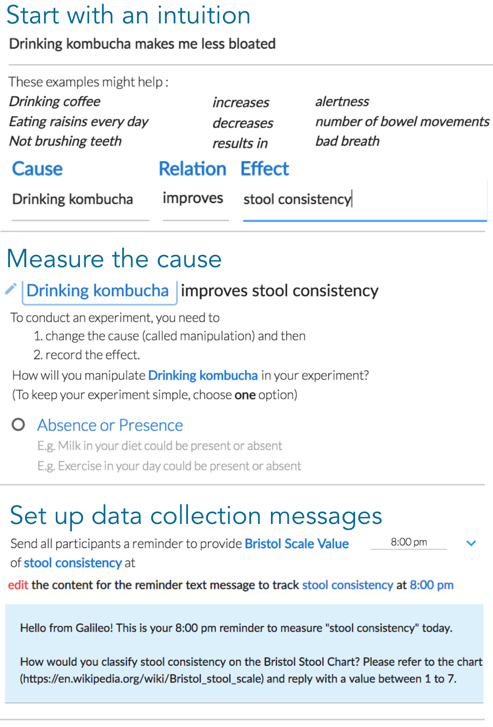
\includegraphics[width=1.0\textwidth]{figures/galileo/galileo-2-design}
%  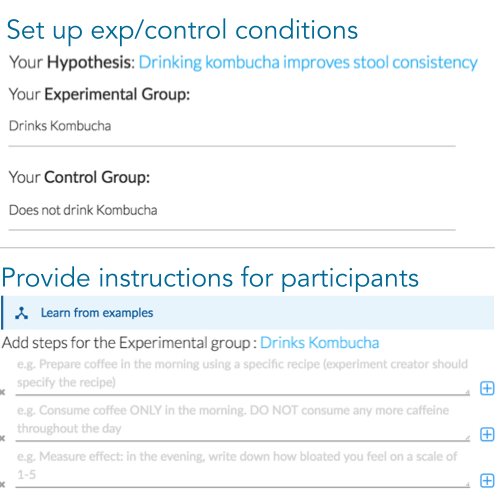
\includegraphics[width=0.48\textwidth]{figures/galileo/galileo-2-design-2}
  \caption[Galileo's design module helps people transform intuitions into experiment designs]
{Galileo's  design module helps people transform intuitions into experiment designs. It walks people through 1) converting an intuition to a hypothesis, 2,3) providing ways to manipulate/measure cause and effect, 4-5) specifying control and experimental conditions, and (not shown) providing inclusion/exclusion criteria.\index{galileo-2}}
  \label{fig:galileo-2}
\end{figure}

Finally, successfully running an experiment requires managing multiple processes such as random assignment, anonymizing participant details, and sending instructions and reminders for data collection.

\subsection{Design-Review-Run: From Intuitions to Investigations}
Galileo requires three roles for each experiment: designer, reviewer, and participant. Galileo offers procedural support for each: 1) a design workflow provides just-in-time training, 2) review with scaffolded questions, and 3) automated routines for runtime activities like data collection. Users form and refine with the help of contextual support and learning resources from the system. 

\subsection{Design an Experiment from an Intuition}
People have many, often poorly-framed, hypotheses. Galileo's design workflow helps people harvest and sharpen them (Figure~\ref{fig:galileo-2}). Examples illustrate possible choices and how they relate; templates provide structure; and embedded videos explicate technical issues. Such procedural support can improve on-task performance~\cite{Pandey2018}. A final self-review step provides an overview of the experiment. To keep the platform safe, the primary author receives daily updates of platform activity. The design workflow does not mandate double-blindness or the use of placebo; designers can choose to specify these details.

%\begin{wrapfigure}[10]{r}{0.5\textwidth}
%  \centering
%  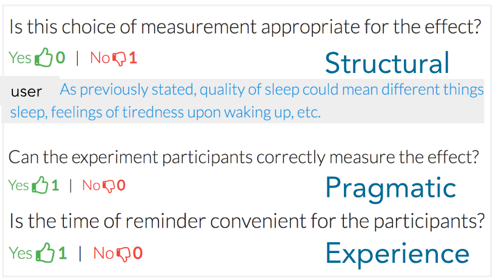
\includegraphics[width=0.5\textwidth]{figures/galileo/galileo-2-review}
%  \caption[Reviewers walk through an experiment providing binary rubric assessments]
%{Reviewers walk through an experiment providing binary rubric assessments. A No response prompts reviewers to provide concerns and suggestions.\index{galileo-2-review}}
%  \label{fig:galileo-2-review}
%\end{wrapfigure}

\begin{figure}[h]
  \centering
  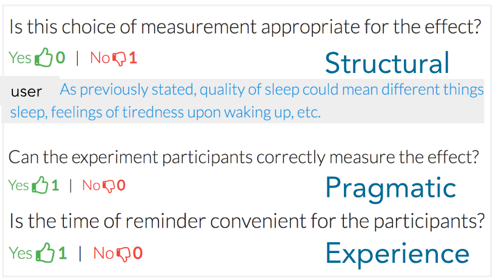
\includegraphics[width=0.5\textwidth]{figures/galileo/galileo-2-review}
  \caption[Reviewers walk through an experiment providing binary rubric assessments]
{Reviewers walk through an experiment providing binary rubric assessments. A No response prompts reviewers to provide concerns and suggestions.\index{galileo-2-review}}
  \label{fig:galileo-2-review}
\end{figure}

\subsection{Review the Design via Feedback from Others}
Galileo experiments require at least two reviews before they can be run. The designer invites the reviewers, who might be online community members, a teacher, or anyone else who can provide useful feedback. Upon receiving reviews, the designer edits the experiment to address any issues. For research purposes, Galileo logs version changes. Reviewers provide both binary assessment and written responses to specific questions (Figure~\ref{fig:galileo-2-review}). These questions cover structure (e.g., accounting for confounds), pragmatics (e.g., measuring the real-world cause/effect), and participant experience (e.g., data reminder time). Reviewers are ineligible to be participants in the same experiment. Similarly, creators may not review their own experiment. 

%\begin{wrapfigure}[17]{r}{0.5\textwidth}
%  \centering
%  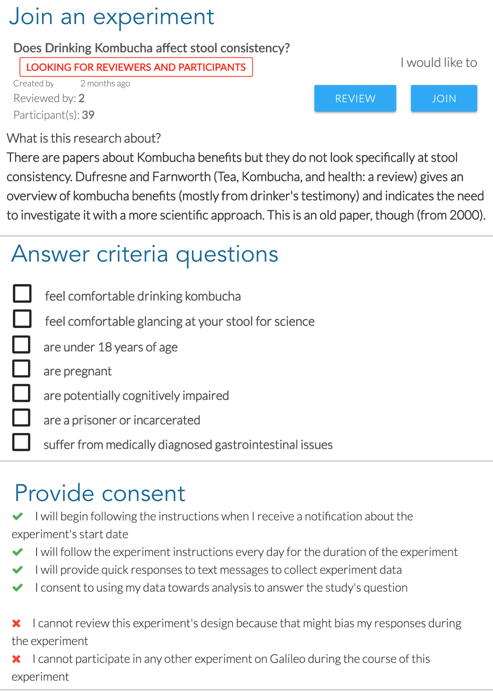
\includegraphics[width=0.5\textwidth]{figures/galileo/galileo-2-run}
%  \caption[Join workflow for participants]
%{Join workflow for participants. 1) Participants can view a list of experiments. When they elect to join one, they 2) answer inclusion/exclusion criteria, 3) consent to following the provided steps, and 4) receive instructions. Participants receive daily, condition-specific requests, and respond with data and/or clarifying questions. \index{galileo-2-run}}
%  \label{fig:galileo-2-run}
%%\vspace{-1pt}
%\end{wrapfigure}

\begin{figure}[!h]
  \centering
  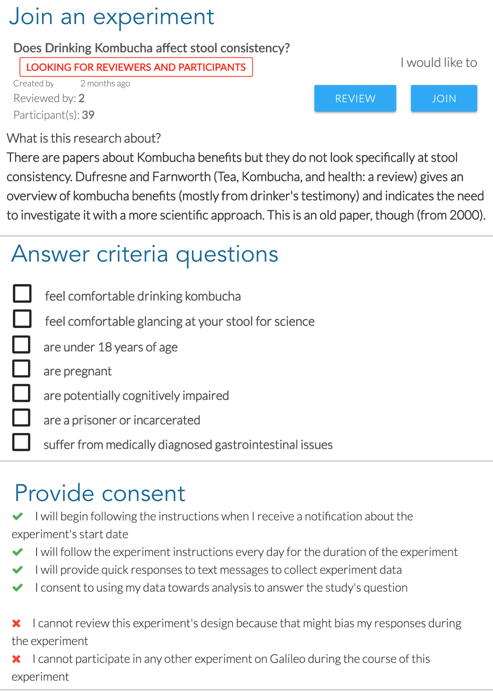
\includegraphics[width=0.5\textwidth]{figures/galileo/galileo-2-run}
  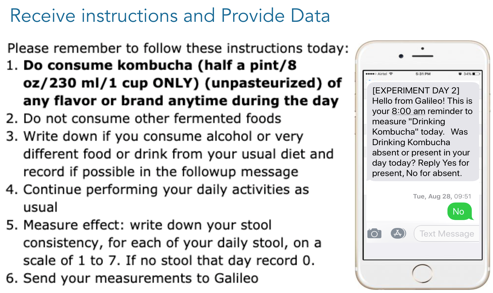
\includegraphics[width=0.5\textwidth]{figures/galileo/galileo-2-run-01}
  \caption[Join workflow for participants]
{Join workflow for participants. 1) Participants can view a list of experiments. When they elect to join one, they 2) answer inclusion/exclusion criteria, 3) consent to following the provided steps, and 4) receive instructions. Participants receive daily, condition-specific requests, and respond with data and/or clarifying questions. \index{galileo-2-run}}
  \label{fig:galileo-2-run}
%\vspace{-1pt}
\end{figure}

\subsection{Run an Experiment using Procedural Support}
To launch an experiment, its designer shares a unique URL with potential participants. Galileo automatically manages four activities to reduce bias and workload:
\begin{enumerate}
\item Randomized placement of people into conditions~\cite{Martin2007}.
\item Maintain a per-experiment participant map ([usernames]$\rightarrow$ [exp$\textunderscore$id]) for anonymity
\item Collect and clean data (sending data collection messages and reminders at time zone appropriate times, parsing the responses, updating participant and experimenter views). 
\item Prompt experimenters to perform tasks when conditions are met (e.g., setting the start date when enough participants have joined or reminding participants with missing data). 
\end{enumerate}

Participation comprises following instructions (e.g., drink kombucha) and providing self-report responses to platform queries (Figure~\ref{fig:galileo-2-run}). The current implementation supports email, SMS, and WhatsApp. Self-reports provide the primary data collection mechanism. Participants can optionally answer follow-up questions that capture contextual insights. Galileo logs responses to a MongoDB database. Galileo presents participant data to experimenters using participant ID rather than real name or username. When the experiment ends, participants receive a summary of results. Participants can anonymously discuss the experiment at the end, so the experimenter can learn from their feedback. 

The experimenter's dashboard lists tasks: answer clarifying questions, remind/thank participants, or look at trends in data (Figure~\ref{fig:galileo-2-run-1}). Experiments have a minimum participation count; there's no upper limit to the number of participants. People who sign up after a cohort begins are added to a waitlist.
The Galileo web application uses the Meteor (meteor.com) framework for synchronization, Jade for the front end (jade-lang.com), Materialize for styling (materializecss.com), and Twilio as the text message gateway (twilio.com).

\begin{figure}[!h] 
  \centering
  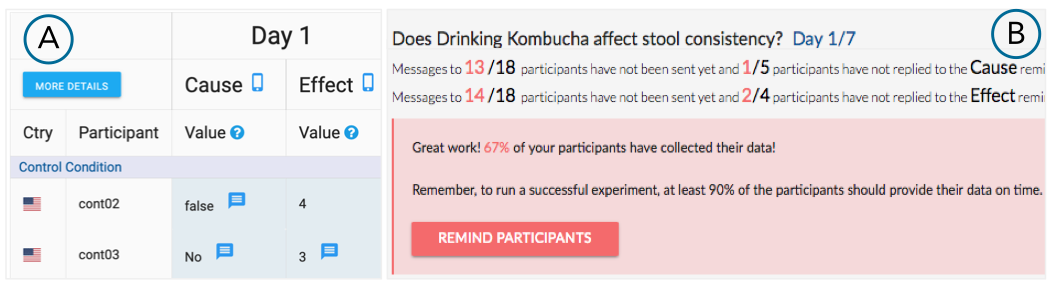
\includegraphics[width=1.0\textwidth]{figures/galileo/galileo-2-run-1}
  \caption[Galileo takes care of many experimenter responsibilities such as random placement of people, sending instructions and reminders, and cleaning and displaying data in both participant and experimenter dashboard]
{Galileo takes care of many experimenter responsibilities such as random placement of people, sending instructions and reminders, and cleaning and displaying data in both participant and experimenter dashboard. The dashboard enables experimenters to A) remind those with missing data; and B) see participants' data; and clarify questions raised by participants.\index{galileo-2-run-1}}
  \label{fig:galileo-2-run-1}
\end{figure}

\subsection{Designing the platform}
More than 80 people have designed and run experiments. The system design evolved over a year of weekly in-person user-centered studies with lead users from different communities including kombucha and self-tracking enthusiasts. The pilot study gathered feedback on the usefulness of the interface items and resources. Students in an undergraduate Psychology class (Introduction to Research Methods) also used Galileo in a 90-minute classroom deployment to rapidly design and review each others'experiments and receive feedback. We provide three examples of how pilot studies informed Galileo's design:

\begin{enumerate}
\item \textit{Embedded written training over videos}: Early versions provided short, online lecture videos as the learning materials. Most users did not watch them end-to-end to extract the step-relevant insight(s). In response, each step's content now offers written examples, which are easier to skim and refer back to. 

\item \textit{Supporting actionable feedback}: For the review interface, early versions only requested binary Yes/No responses similar to popular crowdsourcing platforms; both experiment designer and reviewers found this to be unsatisfactory. Galileo now provides a prompt for actionable feedback whenever the reviewer selects "No" to any question. 

\item \textit{Ease of glancing at participants' data}: Pilot users ran six trial experiments. The idea of a runtime dashboard (Figure~\ref{fig:galileo-2-run-1}A) came from observing experimenter's difficulty tracking participants' data and sending reminders to those who hadn't added their data. Participants struggled with making suitable preparations for a week of experimentation (e.g. buying sufficient kombucha). The system now prompts experimenters to explicitly add preparation instructions that are sent to participants 2 days before the experiment begins. 
\end{enumerate}

\subsection{Integrating Procedural Support in the Design Workflow}
Simple examples of procedural learning are activities like tying your shoes, roasting a chicken, or replacing a door handle. Recipes and instructions convey procedures in written form; demonstrations and hands-on learning make it more interactive. Creative tasks differ from rote procedures in that they require people to generate some artifact themselves.

\subsubsection{Embedding Just-in-Time Support}
Complex activities overwhelm learners' working memory because of their many interrelated pieces~\cite{Engle2002}. Recalling work from previous steps and frequent context-switching are especially taxing~\cite{Gonzalez2004}. Experts mitigate memory demands by integrating multiple elements into conceptual chunks~\cite{Chase1973}. A well-chunked interface can still require knowledge that novices lack. Galileo provides missing knowledge by providing learning materials in the interface. This \textit{in-situ} embedding has three advantages: it is minimal~\cite{Carroll1987}, leverages teachable moments~\cite{Havighurst1953}, and can be ability-specific~\cite{Corbett1997}. Finally, as is good user interface practice, selecting good defaults for each step helps users see an example of appropriate choices. 

Early Galileo users sometimes made poor choices, like listing effects that are difficult to measure. To help guide people, Galileo now presents a short checklist for verifying the choices made in each section. This self-review provides lightweight, just-in-time support.

\subsubsection{Example: Training people to identify a cause}
Controlled experiments seek to identify develop causal understanding by varying just the cause in experimental conditions. Many people do not understand the importance of having this minimal-pairs design, perhaps because they do not have the same issues in mind when thinking about the cause as when thinking about the conditions.

Galileo administers the following process to help designers select conditions that test a causal claim. It provides a simple description in common English with ~3 examples showing the data collection reminder text and times right after the designer decides on the cause and effect metrics. Galileo auto-populates text reminders with readable sentences~\cite{Levy2013} that people can edit. Finally, checklists help people review and improve their work. Such checklists refer to more context-specific challenges of making the experiment simple, safe, and comfortable for participants.
 
Three studies evaluated Galileo's approach: a controlled experiment to test procedural support's efficacy in the design workflow; a field study to test whether people can create structurally-sound experiments based on personal intuitions; and a deployment to test whether people can design and run experiments. 

%%%%%%%%%%%%%%%%%%%%%%%%%%%%%%%%%%%%%%%%%%%%%%%%%%%%%%%%%
\section{Study 1: Experiment Comparing Procedural Support to Videos}
To investigate whether procedural support helps novices design experiments, a between-subjects experiment tested the following hypothesis: \textbf{\textit{Procedural support yields higher quality experiment designs than lecture videos}}. 

Procedural training, when successful, helps people solve unique problems with similar structure. It is perhaps best studied in K-12 mathematics instruction~\cite{Rittle-Johnson1999}. We hypothesize that participants who use interactive procedural support create better experiment designs than those who watch videos on the topic. 

\subsection*{Method}
Participants were randomly assigned to one of two conditions: \textit{Videos} or \textit{Galileo} (Figure~\ref{fig:galileo-6-study}). The \textit{Videos} condition provided a playlist of videos about experiment design from a Coursera MOOC that operationalized the task-specific concepts~\cite{Wobbrock2018}. The \textit{Galileo} condition provided participants access to Galileo. Both provided the same content for creating a structurally-sound experiment. Moreover, participants were provided instructions that the resources (videos/Galileo) described the attributes that their designs should possess. Scripted study instructions ensured the same manipulation. 

The study asked participants to compose an experimental design for a personal intuition of their choosing. Each condition provided informational resources and a means to document their design (videos with a text document, or procedural support with inline text fields). Participants were told that there was no lower or upper time limit. Each session comprised the following steps: consent, design task, survey, and interview. Participants could also use web resources--- such as Wikipedia---and many did. The interview asked participants about confidence in their experiment design abilities and their experience using the system. The interview was tailored to participants' behavior and survey responses: for example, if a participant did not watch some videos, the interviewer asked why. An independent rater (a professor who teaches experiment design) blind to condition rated each participant's experiment using the rubric (Table~\ref{tab:rubric1}).

\begin{figure}[t] 
  \centering
  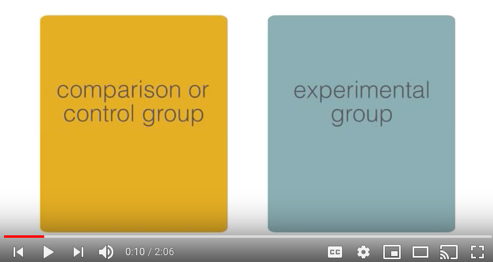
\includegraphics[width=0.48\textwidth]{figures/galileo/galileo-study-1}
  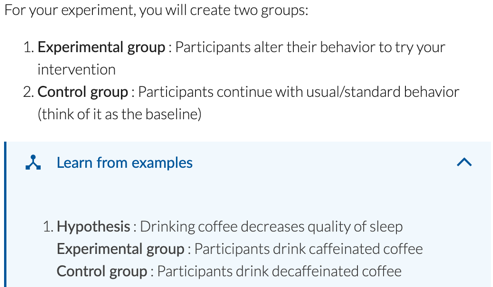
\includegraphics[width=0.48\textwidth]{figures/galileo/galileo-study-2}
  \caption[Two conditions for experiment: \textit{Videos} and \textit{Galileo}]
{Two conditions for experiment. In the \textit{Videos} condition, participants accessed videos about experiment design. In the \textit{Galileo} condition, participants accessed Galileo tool (which included the videos if participants wanted to see them). Both conditions provided the same content. \index{galileo-6-study}}
  \label{fig:galileo-6-study}
\end{figure}

%%%% TABLE 1 %%%%
\vspace{0.25in}
\begin{table}[!ht]
\caption[Demography information for 72 participants (all undergraduate students)] 
{Demography  information for 72 participants (all undergraduate students). Some participants did not complete portions of the survey.}

\vspace{-0.25in}
\begin{center}
\renewcommand{\arraystretch}{1.5}
%\begin{tabular}{c >{\em}c c}
\begin{tabular}{>{\bf}p{1.5in}p{1.75in}p{1.75in}}
\hline
Nationality	&	USA=37		&	China=11\\
			&	No Answer = 6	&	Others = 18\\
Gender		&	Female = 47	&	Male = 24\\
Native English	&	Yes = 38 		&	No = 34\\
Age			&	18-20 = 40	& 	26-30 = 1\\
			&	21-25= 31	&			\\
Ethnicity		&	Asian/Pacific=36 & 	Hispanic/Latino=14\\
			&	White = 11		&	Others=11 \\
Major		&	Biology=12	& 	Psychology=20 \\
			&	Cognitive Sci=12 &	 Others = 20 \\
Used online	& 	Never=28		&	Occasional=16\\
learning		&	1 class=11	&	2-5 classes=12\\
\hline
\end{tabular}
\end{center}
\label{tab:gi-results1}
\end{table}


\subsection*{Participants}
\textit{Recruitment}: 72 participants were recruited from a Western US Research University (Table~\ref{tab:gi-results1}). 11 had no prior experience with experiment design; 61 had taken a course or equivalent. Expertise was counterbalanced across conditions.

\subsection*{Measures}
The independent variable is access to Galileo/videos. The study scored experiments via a 13-question rubric (Table~\ref{tab:rubric1}), and recorded time taken. A blind-to-condition expert (a regular instructor of large, undergraduate courses on experiment design) provided the scores. Qualitative measures included how participants used the tool, where they faced challenges, and a post-experiment survey. A non-parametric Mann-Whitney test assessed the effect of condition on design quality.

%%%% TABLE 2 %%%%
\vspace{0.25in}
\begin{table}[!ht]
\caption[Rubric for design-quality criteria for structure]
{Rubric for design-quality criteria for structure}

\vspace{-0.25in}
\begin{center}
\renewcommand{\arraystretch}{1.5}
\begin{tabular}{p{1.75in}p{3.5in}}
\hline
\textbf{\textit{Hypothesis}: 3 points} & Is the cause/relation/effect specific?  \\
\textbf{\textit{Measurement}: 2 points} & Are the cause and effect manipulated/measured correctly? \\
\textbf{\textit{Conditions}: 3 points}  & Are the control and experimental conditions appropriate? 2 points \\
 & Do the conditions differ in manipulating the cause? 1 point \\
\textbf{\textit{Steps}: 2 points}  & Are experimental steps clear for control/experimental conditions?  \\
\textbf{\textit{Criteria}: 2 points} & Are the exclusion criteria correct and complete? Are the inclusion criteria correct? \\
\textbf{\textit{Overall}: 1 point} & Can the overall experiment be run as is?  \\
\hline
\end{tabular}
\end{center}
\label{tab:rubric1}
\end{table}

%\subsection*{Results}
\subsection{Access to Galileo improved the quality of experiment design}

%\begin{wrapfigure}{r}{0.5\textwidth}
%  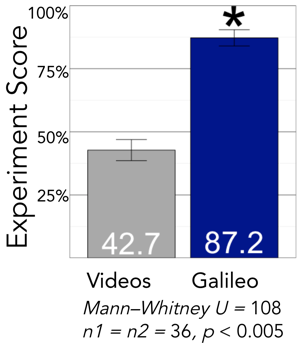
\includegraphics[width=0.5\textwidth]{figures/galileo/galileo-study1-7}
%  \caption[Access to Galileo improved the quality of experiment design]
%{Access to Galileo improved the quality of experiment design\index{galileo-study-1}}
%  \label{fig:galileo-result}
%\end{wrapfigure}

\begin{figure}[h]
\centering
  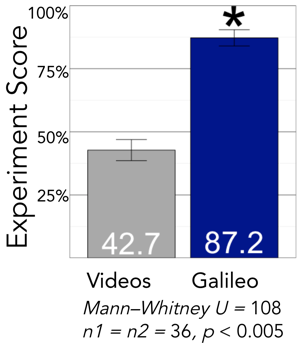
\includegraphics[width=0.5\textwidth]{figures/galileo/galileo-study1-7}
  \caption[Access to Galileo improved the quality of experiment design]
{Access to Galileo improved the quality of experiment design\index{galileo-7-result}}
  \label{fig:galileo-7-result}
\end{figure}

\textit{Galileo} participants created higher-quality experiments (M = 11.3) than \textit{Videos} participants (M = 5.6); Mann–Whitney U = 108, n1 = n2 = 36, p $<$ 0.005 (Figure~\ref{fig:galileo-7-result}). Of the 36 designs rated in the top half, 29 were from \textit{Galileo} condition. \textit{Galileo} participants performed better on five out of six sections (all except hypothesis). There was no significant difference in the amount of time participants spent creating an experiment in the \textit{Videos} condition (M = 30.8 mins) vs \textit{Galileo} (M = 29.0 mins) conditions; Mann–Whitney U = 734, n1 = n2 = 36, p = 0.33 two-sided. 

\subsection*{Discussion}
As Galileo aims to improve tasks like experimental design, Study 1's primary dependent variable was quality (as opposed to learning gains). Online video resources represent a common status quo: contemporary and bite-sized yet still static resources. This comparison enabled us to observe how Galileo's procedural support changed design outcomes. \textit{Videos} participants followed one of two strategies: 1) watch all the videos at once and then begin writing the experiment; or 2) begin designing the experiment and use the videos to fill in the gap when stuck. Like cramming, all-at-once watching floods the mind, perhaps making it difficult to use seen ideas~\cite{kornell2009optimising}. By contrast, the search-when-needed approach interrupts people's flow, replacing the attention on design with a task of locating needed information. \textit{Videos}' lower score and our observations, in conjunction with the literature, suggest contextually-integrated approaches like procedural support increase people's useful adoption of information.
   
Participants reported that the videos were slow and the interface provided sufficient examples. Participants in the \textit{Galileo} condition opened and closed the videos in quick succession. Participants in the \textit{Videos} condition, however, felt that the videos provided a refresher of some concepts they vaguely knew about. Did too much information (e.g. the inclusion of other concepts) in the Coursera course dilute performance? It's possible; accessing the "right" moment in videos is a known research question~\cite{kim2014crowdsourcing}. 

Participants in both conditions expressed a lack of confidence in their chosen cause/effect measures. Some spent over 15 minutes searching for measures: one found a formal sleep-quality scale from Stanford researchers. Participants in both conditions mentioned that they enjoyed reflecting on their lifestyle/health ideas and thinking through how to transform an intuition into an experiment. Participants wished that Galileo was integrated with their class, describing it as "hands on" and "DIY". 

\subsection*{Limitations}
This experiment found procedural support to yield higher-rated designs than watching videos. Important direction for future work will be to compare different approaches to procedural support, and exploring additional measures (e.g., novelty). 

%%%%%%%%%%%%%%%%%%%%%%%%%%%%%%%%%%%%%%%%%%%%%%%%%%%%%%%%%
\section{Study 2: People Design \& Review Experiments Online}
The first study evaluated the efficacy of procedural support for designing experiments. The second study investigated the quality and nature of experiments; specifically, whether people a) create experiment designs that are structurally-sound, demonstrate insights from lived experiences, and have novel ideas, and b) provide useful feedback on experiment designs. 

\subsection*{Method}
Participants used Galileo to design their experiments and review others'. Galileo's landing page described why experiments are important and the importance of citizens' contributions towards making discoveries. Upon logging in, participants could design an experiment (see Figure~\ref{fig:galileo-2}), review existing experiments (see Figure~\ref{fig:galileo-2-review}), or join an experiment (see Figure~\ref{fig:galileo-2-run}). 

\subsection*{Recruitment}
Participants were recruited via online publicity. One recruitment focus was people curious about the microbiome because it is a domain where lived experience may inspire intuitions, and the science is nascent~\cite{McDonald2018a}. Galileo was promoted on the American Gut's and their collaborators' Facebook and Twitter pages. Galileo was added as a project on Open Humans (openhumans.org), posted on multiple subreddits pertaining to health and lifestyle, and introduced as an optional activity in assignments on the Gut Check Coursera MOOC~\cite{Knight2016}. Participation was voluntary and unpaid. 


%%%% TABLE 3 %%%%
\vspace{0.25in}
\begin{table}[!ht]
\caption[Rubric for design-quality criteria for Structure, Content, and Novelty]
{Rubric for design-quality criteria for Structure, Content, and Novelty}


\vspace{-0.25in}
\begin{center}
\renewcommand{\arraystretch}{1.5}
\begin{tabular}{p{1.5in}p{4in}}
\hline
\textbf{Structure} &  \textit{Described in Table~\ref{tab:rubric1}} \\
\textbf{Content}  & \\
~~\textit{Personal?} & Did the hypothesis draw from lived experience? \\
~~\textit{Popular?} & Is the world already curious about this hypothesis (e.g. discussions on online fora)?  \\
~~\textit{Insightful?} & Does the hypothesis link to existing science?  \\
\textbf{Novelty}  &  Is there a chance the world will learn something: absence of published research for this question?\\
\hline
\end{tabular}
\end{center}
\label{tab:rubric2}
\end{table}

\subsection*{Measures}
Measures comprised structure, content, and novelty of experiment designs (Table~\ref{tab:rubric2}) and usefulness of reviews. Raters with training in experiment design independently rated participants' work, then discussed them to form a shared view of assessment. Next, each independently rated all experiments. The final score is the mean of their independent ratings. Moderate reliability was found between the two raters' measurements~\cite{koo2016guideline}; m(ICC) = .62, 95\% CI [.45, .75], (F(64,64)= 4.33, p$<$.001. 

Structure measures whether the design is correct and includes appropriate components. Content measures the subject matter of the idea driving the experiment design; it was rated as personal focus, popularity, and insightfulness of the hypothesis. Novelty was assessed as the potential to create new knowledge and operationalized as the lack of research papers about the specific hypothesis. Raters were instructed to assign points for a component (say hypothesis) if the experiment provided appropriate details about it. For example, the hypothesis \textit{Text message reminder increases consumption of recovery snack} was rated to have a specific cause, a specific effect, and a clear relation between the two, while \textit{Eating too much energy causes disturb [sic] sleep cycle} did not have a clear cause or effect. \textit{Ingesting non-local food results in poor evacuation of fecal matter} '' was rated as novel because no published research addresses this (as per Google Scholar). Broad or vague hypotheses related to well-studied topics were not deemed novel (e.g. \textit{Going to college increases grades}).

54 users from 16 countries created 66 complete experiment designs (Mdn=27 minutes). 37 users provided 205 descriptive review comments. Latest versions of complete experiment designs were scored as described above; incomplete experiments and older versions were removed from analysis. 

\subsection*{Results}
%\subsubsection{People Designed Structurally-Sound Experiments, and Drew from Personal Intuitions}
\subsection{People Design Structurally-Sound Experiments, and Draw from Personal Intuitions}
The mean score for the experiment was 10.3/13. On average, people scored higher than 75\% on 8 of 13 measures. 38\% of experiment designs came for people's lived experiences; e.g., \textit{eating yogurt makes a person have a more regular bowel movement}. Personal health and performance were big draws: 90\% of experiments sought to improve a health outcome. 

\begin{figure}[h]
\centering
  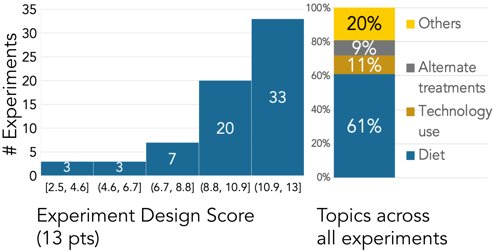
\includegraphics[width=0.7\textwidth]{figures/galileo/galileo-study2-1}
  \caption[Results: Most experiments were structurally-sound and drew from personal experiences]
{A) Most experiments were structurally-sound, scoring high on the structure rubric. B) Most experiments drew from personal experiences \index{galileo-8-result}}
  \label{fig:galileo-8-result}
\end{figure}

51\% of the experiments were rated as popular; their hypotheses were discussed on other online fora; e.g., \textit{having dry mouth (or Sjogren's Syndrome) promotes the growth of less beneficial gut microbes}. Common themes included diet (dietary styles, alcohol, fermented foods), technology use (social media, laptop, mood) and alternative treatments (homeopathy), and health (sleep, pain, gut issues) (Figure~\ref{fig:galileo-8-result}). Apart from being structurally-sound, the best experiment designs shared two features: they shared a personal experience and linked to known research. For example, a user designed an experiment to test yogurt's effect on bowel movement and shared their motivation: 

\textit{\say{For several months I have been producing Yogurt. This is fermented using commercial probiotics, Probiotic-10. My intuition was that since various microbe species were active in the making of the yogurt, this product can help relieve of the various digestive problems one persona can have. It happens that one of my sons was diagnosed with Ulcerative Colitis. among other things he was losing weight rapidly. After several weeks of consuming probiotics and/or the yogurt, he begun to recover.}}

17\% of hypotheses had novel insights that no published research addresses. For instance, \textit{Avoiding foods high in lectins cures long-term post-infectious diarrhea} and \textit{Drinking kombucha regularly reduces joint inflammation/arthritis symptoms} are both hypotheses of interest to citizens and microbiome researchers alike.

%\begin{wrapfigure}[8]{r}{0.5\textwidth}
%\centering
%  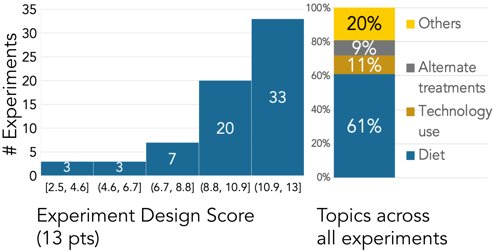
\includegraphics[width=0.48\textwidth]{figures/galileo/galileo-study2-1}
%  \caption[Results: Most experiments were structurally-sound and drew from personal experiences]
%{A) Most experiments were structurally-sound, scoring high on the structure rubric. B) Most experiments drew from personal experiences \index{galileo-study2-1}}
%  \label{fig:galileo-result2}
%\end{wrapfigure}

\begin{figure}[h] 
  \centering
  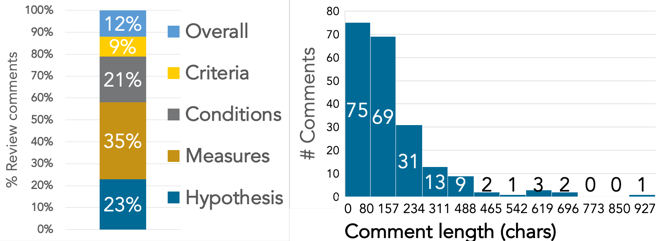
\includegraphics[width=0.66\textwidth]{figures/galileo/galileo-study2-2}
  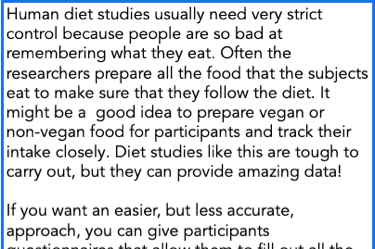
\includegraphics[width=0.33\textwidth]{figures/galileo/galileo-study2-3}
  \caption[Result: Review comments were distributed across all components of experimental design]
{Summary of review A) Review comments were broadly distributed across all components of experimental design. B) Review comments ranged from 3 chars "yes" to 871 char long descriptions. C) The longest review comment described multiple problems with an experimental design while providing numerous actionable suggestions. \index{fig:galileo-9-result}}
  \label{fig:galileo-9-result}
\end{figure}

%\subsubsection{Reviewers Use Domain Knowledge to Improve Designs and Advocate for Participant Experience}
\subsection{Reviewers Use Domain Knowledge to Improve Designs and Advocate for Participant Experience}
158 review comments (77\%) were rated useful; incorporating them would improve the experiment. Average comment length was 140 characters ranging from 3 characters (\textit{yes}) to 871 characters (Figure~\ref{fig:galileo-9-result}B,C). Most comments were direct responses to a rubric question hinting that the review interface helped people focus on the salient parts of an experiment design.

The most common comments sought improving structural correctness (38\%) by requesting specific details. For example, one reviewer questioned an experiment's choice of Likert scale for mood saying, \textit{A simplistic Likert scale seems like a bad idea. There has to be something better than this. At least a couple questions? Like, optimism, excitement, depression, anxiety?}. Reviewers provided the most comments (54\%) about the hypothesis and cause \& effect measures. People advocated for improving participant's experience (18\%). Suggesting better data collection messages and times was a popular theme. We present two examples: 1) \textit{People are not very good at remembering what they eat. Maybe an App like MyFitnessPal would be useful since it would allow participants to track all the food they eat without having to remember for too long}, and 2) \textit{How long do they [experiment participants] have to answer? What if they're eating dinner and can't get to it until 9pm?}.

14\% of comments demonstrated domain-specific knowledge E.g., one reviewer pointed out a conceptual mistake about a Type-1 diabetes experiment: \textit{A1C is measured monthly and won't change after 1g. You mean the BG value?} A1C refers to the average blood glucose value average levels over the past 3 months that is less susceptible to short term changes. BG here refers to the blood glucose value that depends on immediate glucose intake (among other factors). Surprisingly, reviewers barely drew from their personal experience when suggesting improvements (or at least, did not explicitly mention this was their personal experience). Some comments drew on counterfactual reasoning while thinking about how participants might "hack" an experiment. A comment on an experiment about social media use and steps walked asked, \textit{…the timing of this [reporting steps taken] vs. social media use measure is off and that makes me worry about intervening use throwing things off (e.g. \textit{\say{phew! I've reported my facebook for the day, now I can go use it}?}})

%%%%%%%%%%%%%%%%%%%%%%%%%%%%%%%%%%%%%%%%%%%%%%%%%%%%%%%%%
\section{Study 3: People Design, Review, \& Run Experiments}
The previous two studies found that people generated novel, structurally-sound experiments. Might they successfully run experiments with others? Participants from three communities---Kombucha, Open Humans, Beer---designed and ran experiments (Figure~\ref{fig:galileo-10-result}).  

\textbf{Does drinking Kombucha improve stool consistency?} Kombucha is a fermented tea drink popular in many parts of the world. Fermented foods (miso, yogurt, ayran, kefir) have been a staple in many cultures for thousands of years~\cite{Chilton2015}. While there is widespread belief that kombucha ``benefits the gut", there is little published empirical evidence for these claims~\cite{Ernst2003}. The experimenter hypothesized that kombucha supplies beneficial probiotics that help maintain normal stool consistency, and designed a between-subjects experiment.

\begin{figure}[h] 
\centering
  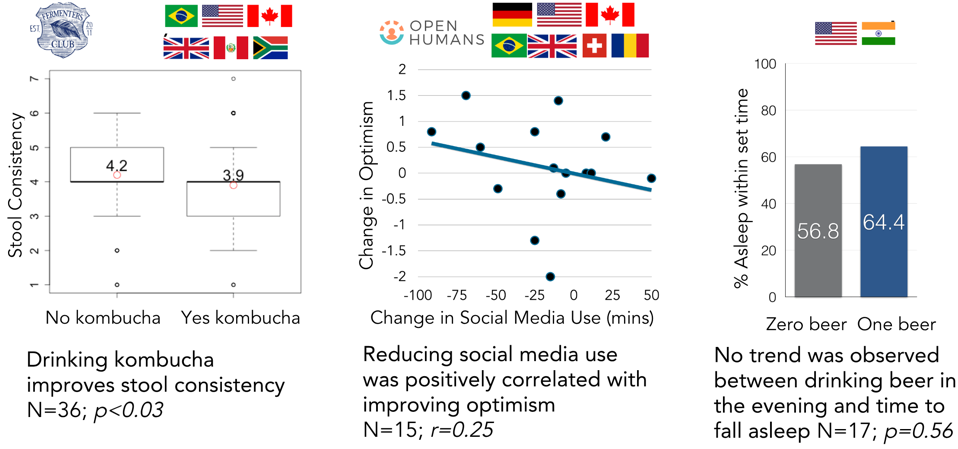
\includegraphics[width=1.0\textwidth]{figures/galileo/galileo-study3}
  \caption[Three communities---Kombucha, Open Humans, Beer---designed and ran experiments]
{Three communities---Kombucha, Open Humans, Beer---designed and ran experiments; each ran for a week. The flags represent participants' nationality. \index{galileo-10-result}}
  \label{fig:galileo-10-result}
\end{figure}

\textbf{Does reducing social media time increase optimism}? Open Humans enables people to contribute personal data (e.g., genetic, social media, activity) for donation to research projects (openhumans.org). An experimenter investigated the relationship between social media and mood. Curious about the popular Facebook contagion study~\cite{Coviello2014}, an Open Humans member (openhumans.org) created a between-subjects experiment to investigate social media and optimism.

\textbf{Does drinking a beer in the evening help people fall asleep}? Some people believe that a pint of beer in the evening helps them sleep by relaxing them; others think alcohol disturbs their sleep~\cite{Ph.D.}. Alcohol helps people fall asleep but disrupts the REM cycle~\cite{Ebrahim2013}. Still, it can be more convincing to see the evidence oneself. The experimenter (a graduate student) tested the effect of beer on sleep time with a between-subjects experiment. 

%%%%%%%%%%%%%%%%%%%%%%%%%%%%%%%%%%%%%%%%%%%%%%%%%%%%%%%%%
%\subsection*{Results}
%\subsubsection{Before the Experiment: Design, Review, Pilots, and Finding participants}
\subsection{Before the Experiment: Design, Review, Pilots, and Finding participants}
From initial design to launch, 37 (kombucha), 13 (Open Humans), and 11 (beer) days elapsed. Each experiment ran for a week.

\textit{Design and Review}: None of the experimenters had previously designed and run an experiment with people. All knew some concepts about experiment design; two have PhD degrees (in biology and ecology) and one is enrolled in a Computer Science PhD program. The experimenters are Brazilian, German, and US nationals. While the three experimenters had lived experience of their experiment's topic, they had never scientifically studied it.

Reviewers provided a total of 104 boolean answers and 32 detailed comments. Comments focused on two themes. First, reviewers helped make the hypothesis and measures more specific; e.g., an experimenter started with the question \textit{\say{Does drinking a beer in the evening help you get to bed on time?}}; the reviewers nudged the experimenter to creating the more specific hypothesis: \textit{\say{Drinking a 5\% ABV (+-0.5\%) beer between 6PM and 8PM local time helps people fall asleep no more than 30 minutes past their desired bed time}}. A reviewer criticized Kombucha experiment's 5-point Likert scale for bloatedness as overly vague. In response, the experimenter found and adopted the Bristol stool chart---a picture-based scale that is the industry standard~\cite{Wikipedia2018}. Second, reviewers suggested improving data quality by instructing participants to skip confounding activities. For example, reviewers pointed out that caffeine and alcohol interact. The experimenter addressed this in instructions asking participants to abstain from coffee and alcohol. All issues that reviewers raised were tightly connected to Galileo's review rubric (Figure~\ref{fig:galileo-2-review}). At the end of review, the three experiment designs used appropriate measures, provided a minimal-pairs design, tracked confounds, and provided appropriate criteria for participation.

\textit{Pilots}: Three lessons emerged. First, some participants were loath to look at their stool. Since viewing one's stool is necessary, the experimenter added an inclusion criterion enforcing this. Second, some participants reported eating other fermented foods in the process; the experimenter modified the instructions for participants to not consume these. Third, after failing to recruit sufficient participants, the experimenter collaborated with a kombucha fermenter in an American city who knew more kombucha enthusiasts. Before testing for the effect of social media, an Open Humans member piloted a study on the effect of 30 extra minutes of aerobic exercises on sleep. However, potential participants were loath to alter their lifestyle this dramatically, and so the experimenter abandoned the study.
 
\textit{Finding participants}: The Kombucha experimenter publicized the experiment on Instagram, Twitter, and newsletter; they also created a poster, and reached out to enthusiasts in their city in Brazil and an American city. The Open Humans experimenter recruited on social media, a mailing list, and the Open Humans Slack channel. The beer experimenter reached out to peers interested in community experimentation and/or the effects of alcohol. At least one potential participant in each of the three experiments was excluded because of inclusion/exclusion criteria. 

%\begin{wrapfigure}[13]{r}{0.5\textwidth}
%\centering
%  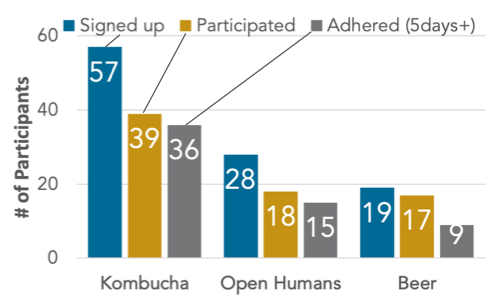
\includegraphics[width=0.48\textwidth]{figures/galileo/galileo-study3-1}
%  \caption[Dropout and Adherence Rates across the three experiments]
%{Dropout and Adherence Rates across the three experiments. After signing up, a smaller fraction of people participated in Kombucha (68\%) and Open Humans (63\%) experiments than Beer (90\%). However, those who participated reported greater adherence in Kombucha (92\%) and Open Humans (83\%) compared to Open Humans (50\%). Reasons for non-adherence included being busy, annual leave, and brewers needing to check on the taste of Kombucha. \index{galileo-study3-1}}
%  \label{fig:galileo-result3-1}
%\end{wrapfigure}

\begin{figure}[h]
\centering
  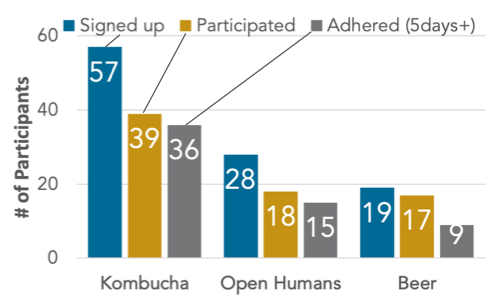
\includegraphics[width=0.7\textwidth]{figures/galileo/galileo-study3-1}
  \caption[Dropout and Adherence Rates across the three experiments]
{Dropout and Adherence Rates across the three experiments. After signing up, a smaller fraction of people participated in Kombucha (68\%) and Open Humans (63\%) experiments than Beer (90\%). However, those who participated reported greater adherence in Kombucha (92\%) and Open Humans (83\%) compared to Open Humans (50\%). Reasons for non-adherence included being busy, annual leave, and brewers needing to check on the taste of Kombucha. \index{galileo-11-result}}
  \label{fig:galileo-11-result}
\end{figure}

%\subsubsection{During the Experiment}
\subsection{During the Experiment: Retention and Data Collection}
\textit{Retention}: 57 people signed up for the kombucha experiment; 36 completed it (68\%). Retention rates were similar for the Open Humans experiment (63\%) and higher for beer (90\%) (Figure 11). 78\% of dropouts occurred in the first 48 hours. The reasons participants reported for dropping out included lack of interest, holidays, and work travel.
Adherence: Kombucha garnered 76\% adherence: 86\% for days of no kombucha, and 70\% when asked to drink kombucha. Most Open Humans participants reported high adherence, cutting social media use in half or more (Figure~\ref{fig:galileo-11-result}). Each day, an average of 54\% of participants in the beer experiment reported following the condition requirement (drinking 1 or 0 beers by 8PM). 15 of 17 failed to comply on at least one day.

%\begin{wrapfigure}{r}{0.5\textwidth} 
%\centering
%  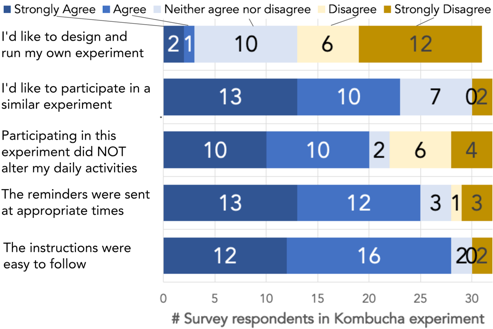
\includegraphics[width=0.5\textwidth]{figures/galileo/galileo-study3-2}
%  \caption[Participants in the kombucha experiment reported an overall positive experience]
%{Participants in the kombucha experiment reported an overall positive experience expressing an interest to participant in another similar experiment (23/32). Most found the instructions easy to follow (28/32) and the reminders sent at appropriate times (25/32). \index{galileo-study3-2}}
%  \label{fig:galileo-result3-2}
%\end{wrapfigure}

\begin{figure}[h]
\centering
  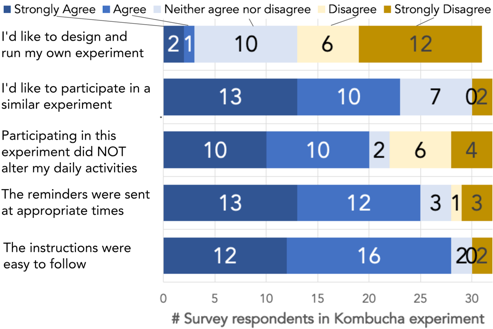
\includegraphics[width=0.7\textwidth]{figures/galileo/galileo-study3-2}
  \caption[Participants in the kombucha experiment reported an overall positive experience]
{Participants in the kombucha experiment reported an overall positive experience expressing an interest to participant in another similar experiment (23/32). Most found the instructions easy to follow (28/32) and the reminders sent at appropriate times (25/32). \index{galileo-12-result}}
  \label{fig:galileo-12-result}
\end{figure}

Some participants disclosed confounds and reasons for non-adherence. For example, drinking alcohol was a reported confound, because it might affect kombucha's impact on the body. Similarly, participants' non-adherence reports included scheduled disruptions like travel and holidays and work responsibilities like brewers needing to check on the taste of kombucha. Non-adherence for the beer experiment included drinking wine rather than beer, drinking after 8PM, drinking more than one beer, or not drinking in the drink-one condition.

\textit{Data Collection}: Most American participants selected text solicitations (86\%); participants elsewhere received email solicitations due to varying regulations around automated text messages (e.g., replying to an automated text message in Brazil or India is infeasible since the source number is masked). 56\% of participant responses came within 30 minutes of the solicitation; 21\% of responses took more than 90 mins. Participants sparingly responded to follow-up questions. Experimenters used the remind participant button 2 (kombucha) and 3 (Open Humans) times to remind participants with missing data.

\textit{Clarifying questions}: The experiment requested that all participants adhere to the protocol as much as possible without harming their health. Participants could ask the experimenter (via the platform) if confused. Participants' clarifying questions focused on measurements (e.g., measuring stool consistency once during the day or multiple times) and specific lifestyle choices (e.g., consuming probiotics while drinking kombucha?). Participants in kombucha experiment reported an overall positive experience (Figure~\ref{fig:galileo-12-result}).

%%%%%%%%%%%%%%%%%%%%%%%%%%%%%%%%%%%%
\section{Reflection}
Our results point at three challenges in democratizing experimentation: 1) the three experimenters had advanced degrees, 2) two of the three completed experiments were underpowered, and 3) experiment participants demonstrated varying levels of adherence. 

\subsection{Do successful citizen-led experiments require prior expertise?}
While an advanced degree is not a prerequisite, having one confers an advantage. This is unsurprising; contributions to open access web platforms are rarely uniform across educational levels. MOOCs are disproportionately completed by learners from more-affluent and better-educated neighborhoods~\cite{hansen2015democratizing}, and 73\% of citizen scientists and Wikipedia contributors have advanced degrees~\cite{national2018learning, Wikipedia} . 

Why were all three experiments run by people with advanced degrees? One reason could be self-selection: those without prior expertise in experimentation might have opted out of running an experiment. This is weakly supported by data: all 36 participants in the kombucha experiment enjoyed the experiment and wanted to participate in more experiments (Figure 14). However, only two participants wanted to design and run follow-up experiments; both have an advanced degree. While simply asking people to contribute might work for traditional citizen science projects, experimentation might be a bigger leap. We suggest two improvements. First, reduce effort by providing ready to run experiments; common health and lifestyle topics such as coffee consumption and sleep might be good candidates. Running a sample experiment enables people to pilot the platform before testing their ideas while also potentially making them comfortable with the idea of experimentation itself. Second, support a growth mindset~\cite{dweck2016having}: e.g. the platform can emphasize that anyone can learn how to run an experiment.

Another reason for experimentation by those with advanced degrees could be their awareness of potential participants. All three experimenters had access to people who were interested in similar topics; e.g., the Open Humans experimenter received both participants and feedback for their idea from the group's slack community. Such \textit{affinity spaces} are known to provide potential participants as well as social support~\cite{gee2005semiotic}. To tackle this, the design workflow can nudge the creator to start their experiment design by thinking of topics relevant to their social connections.

\subsection{Guidance Techniques to Enable Citizens to Recruit Others}
Two of the three completed experiments were underpowered. Citizen experimenters learned what many scientists know: recruiting participants is time-consuming. This suggests that a good experimental design is not enough and recruiting is the next challenge for citizen scientists on their way to develop meaningful knowledge. While the absence of shared knowledge with experts can sometimes give novices' work a boost (e.g. identifying green pea galaxies on Galaxy zoo), it's less useful when the lack of knowledge is a hindrance. Tools for training and collaboration can help by clearly conveying the importance of getting enough participants; enabling experimenters estimate what "enough" is; and providing sources and strategies to recruit participants.

Citizen experimenters aren't as ardent about sufficient participation numbers as professional scientists. One important piece of technical knowledge is performing power analysis before running the experiment. Additionally, following the lead of data journalists~\cite{Gray2012}, conveying results through real-world effect sizes---such as additional years you'll live---might be useful. Moreover, the experimenter need not find all the participants by themselves. Akin to a Clinical Research Coordinator, a separate recruitment role can help the experimenter rope in others to help out. Participants signed up for an experiment can also assist by suggesting others ala snowball sampling.

How might we help increase participation? Common reasons why people join \textit{expert-led} experiments include~\cite{NIH2015}: to help find an answer to a question that personally affects them, to gain access to potential treatments, and for credit or monetary compensation. Moreover, the trust placed in institutional researchers might not extend to citizen experimenters~\cite{Cooper2014}. 

Adherence, however, remains a challenge. The opportunity to contribute to science is exciting (e.g. kombucha experiment participants mentioned this as a motivation). While altering one's lifestyle for a day might not be very difficult for many people, doing the same for a week (or more) might be tedious enough to entirely avoid participating, drop out after signing up, or not adhere to the instructions.

Drawing on findings from social computing and crowd-funding~\cite{hui2014understanding, Karkar2017a}, we suggest four remedies to improve both participation and adherence numbers: 1) increase participant trust by sharing more information about the experiment's goals, approximate effort expected, and the experimenter's biography; 2) implement \textit{activation thresholds} to make social reciprocity explicit for group activities and to reduce potentially wasted efforts~\cite{cheng2014catalyst}; 3) leverage participation from communities with already strong ties and common goals; 4) allow people to pre-register for topics of interest so they might join relevant experiments created at a later date~\cite{bernstein2011crowds}.

Our study did not provide experimenters or participants monetary compensation. Consequently, people's motivation is more intrinsic, which has benefits~\cite{NationalCouncilforVoluntaryOrganisations2018} (e.g. telling people the importance of their work improves performance~\cite{Chandler2013}), but also empirically shows a high dropout rate. Compensation may help some citizen science experiments. 

%%%%%%%%%%%%%%%%%%%%%%%%%%%%%%%%%%%%%%%%%%%%%%%%%%%%%%%%%
\subsection{Design Implications for Knowledge Work}
We suggest three heuristics for systems that chunk complex knowledge work: separate roles, provide interactive guidance, and facilitate iteration. These ideas extend minimalism to design learning experiences~\cite{VanderMeij1995}. 

\begin{enumerate}
\item \textit{Identify roles}. People, especially novices, often struggle to get started. Role-based approaches confer three benefits: clean delineation of responsibilities improves chances of task completion, clustering similar tasks reduces overhead and increases consistency; and people can decide their contribution levels. Procedural support operationalizes minimalism by co-locating tailored learning resources with specific steps.

\item \textit{Provide procedural support for just-in-time domain-expertise}. A diverse audience might not interpret instructions consistently, or fail to translate textbook definitions to practice. Our results show that people are good at interpreting procedural support (like examples) for their use case. Creating such learning resources using the crowd or even learners themselves could reduce the effort needed~\cite{Kim2014c}. 

Checklists, cognitive aids, and tutoring systems exploit chunking as a means of onboarding new participants in a community of practice. For checklists, these chunks are usually static and expert-designed. A powerful benefit of interactivity is the opportunity for personalization. To reduce the time spent designing scaffolds and workflows, reuse lessons from other tools.
 
Our first two heuristics focus on the authoring piece. Our third heuristic focuses on the reviewing piece. In contrast with cognitive aids and tutoring systems that "bake in" knowledge, our review step---like learnersourcing~\cite{Kim2014c}---leverages the crowd for customized feedback. Structured reviewing---like Galileo---simultaneously discourages the lazy shortcut of superficial reviewing, and lowers the cognitive burden of providing deep, actionable feedback. 

\item \textit{Handle errors using iterations}. Most first drafts have errors. Feedback can be provided by experts~\cite{dow2012shepherding, schon1984reflective}, peers~\cite{Boud1995, Kulkarni2015b}, software~\cite{Dantoni2015}, or even oneself~\cite{Boud1995, schon1984reflective}. Support iterations and pre-task training can counter concerns of superficial reviews. Why? Scaffolded questions and checklists help people reflect on their work at every step, especially when the system fails to automatically tackle inconsistencies for open-ended work.
\end{enumerate}

%%%%%%%%%%%%%%%%%%%%%%%%%%%%%%%%%%%%%%%%%%%%%%%%%%%%%%%%%
\subsection{Do Citizen  Experiments Benefit or Harm Society?}
One challenge of modern life is the increasing layers of social and technical infrastructure that separate the creation of knowledge from its everyday use. This divorce makes it difficult to wisely assess and use knowledge. This paper has outlined the positive potential for citizen designed experiments, a greater range of perspectives, participation, and understanding. It's worth considering the risks. The primary concern we have is that a poorly designed experiment with a faulty conclusion influences people in fraught ways.
 
At its best, over time scientific experiments expand human knowledge and correct mistakes when they occur. However, sometimes the popular press reports a headline-grabbing result that is inaccurate, but not the subsequent correction and elaboration. Particularly with science, when ideas are newsworthy but low-quality, people can incorporate misguided ideas in a way that be difficult to dislodge. Perhaps the most notorious example is the (debunked) claim that vaccines, especially MMR vaccine, cause autism by disrupting the body's microbial composition  and/or introducing harmful chemicals. At a time of rising autism diagnoses, this claim terrified parents and continues to impede childhood vaccination more than two decades later . Furthermore, the 20th century offers many examples of pervasively-adopted chemicals (such as lead in paint and gasoline, and asbestos in buildings) that were later found to be toxic. Wakefield's publication linking MMR vaccine to autism (later retracted) was a serial case study~\cite{Godleec7452}, not an experiment. While sharing case studies can help identify valuable leads for further study, the small size and biased selection create enormous risk of confounds and spurious relationships. (In this case, unidentified correlated timing in the measures and undisclosed financial ties by the author further clouded the picture.) Currently, most readers cannot fully grasp the evidentiary difference between a small case study and a rigorous controlled experiment. Our hope is that democratizing the doing of science may help the public interpret science news and reduce the risk of leaping to conclusions.

Because not all experiments are appropriate for people to run, some gatekeeping of citizen experiments might be necessary. 62 of 66 complete designs were posted online on Galileo for others to view; the primary author took 4 down because the research team identified them as risky. For example, one removed design sought to investigate the effect of colloidal silver on cognitive performance. There is a community that believes colloidal silver (tiny particles suspended in liquid) to have beneficial properties~\cite{DanaLewis}. While the designer may be well-intentioned, consuming colloidal silver can cause irreversible damage such as skin discoloration, and the NIH has sued manufacturers for misleading claims~\cite{Health2018}. Galileo offers keyword triggers for alerting both the designer and the research team of possibly dangerous experiments. For example, an experiment containing "cancer" or "CBD" triggers an email to the research team; use of the word "cancer" indicates potential health risks for participants (who might be cancer patients) while "CBD" indicates potential legal risks across many places around the world.

%%can people actually find answers to questions suggested by experts who are too busy to run that experiment themselves -- complementing clinicians 1. see work around patient-led experimentation

Sifting through ideas expressed by people for experimentation, we believe citizen experiments seem well suited for ideas that meet three criteria; they must 1) be scientifically tenable, 2) combine high excitement with low efforts, and 3) provide zero to no risk. Scientifically tenable means that the experiment answers a gap in research literature, minimizes placebo effects, and yields results in a week with a high likelihood. To be low-effort, all the experimental steps (including reporting data) should be easy to understand and perform. Finally, the experiment should not provide any cause of harm to participants and it should be legally and ethically permissible across countries and cultures. As a crude beginning, this can be operationalized as the existence of numerous anecdotes about potential upsides with none or well understood downsides. For instance, bee venom reduces Lyme disease symptoms (an idea proposed on the platform) is an idea with anecdotal benefits but the existence of venom implies non-trivial possibility of self-harm.

%%%%%%%%%%%%%%%%%%%%%%%%%%%%%%%%%%%%%%%%%%%%%%%%%%%%%%%%%

This paper investigated citizen-led experimentation with novel procedural support. Three empirical investigations tested this approach. For us, the most striking result is that online volunteers collaboratively performed scientific experimentation without any expert help by drawing on their lived experience. Our work also illustrates the challenge of helping novices successfully execute a complex knowledge task. Specifically, finding and retaining participants and making the platform accessible to a broader audience emerged as key challenges. With systems that enable citizen-led experimentation, people can potentially match scientists' knowledge with their lived experiences to create insights both for themselves and for the scientific community. More generally, we hope that our work suggests ways to build systems that provide just-in-time domain expertise for knowledge work. Such systems can enable novice-led work that is personally meaningful, and situated in people's lived experiences.

This chapter, in part, includes portions of material as it appears in  the submitted paper \emph{Galileo: Procedural Support for Citizen Experimentation} by Vineet Pandey, Tushar Koul, Chen Yang, Daniel McDonald, Mad Price Ball, Bastian Greshake Tzovaras, Rob Knight, and Scott R. Klemmer. The dissertation author was the primary investigator and author of this paper.

